\section{Surface Geometry}
This section covers the basics introduced in how to represent shapes in a computer.
\subsection{Notes}
\begin{itemize}
	\item Graphics Pipeline: It refers to the sequence of steps used to create a 2D raster representation of a 3D scene. It is the process of turning a 3D model into what the computer displays. 
	\item Vertex: A point with three numbers representing its XYZ position in a plane
	\item Edge: An edge is the difference between two vertices; the segment connecting them
	\item Surface: A closed set of edges representing a face of a 3D object
	\item Polygon: A shape in space usually representing by a set of surfaces (other methods listed below)
	\item Polygon Table: A table containing a set of either vertices, edges and/or surfaces that is used to define the boundaries of a polygon. This is one method to define Polygons.
	\item Delaunay Triangulation: Given a set P of points in a plane, creates a triangular mesh DT(P) such that no point in P is inside the circumcircle of any triangle in DT(P).
\end{itemize}
   \begin{figure}[!htb]
	\center{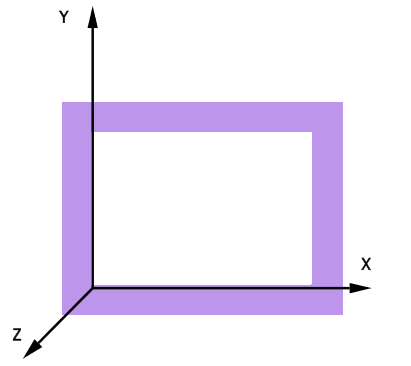
\includegraphics[width=3cm]
		{graphics/rhcoords}}
	\caption{\label{fig:rhcoords} Coordinate system assumed throughout module}
	\end{figure}
The default coordinate system assumed is right-handed: the positive x and y axes point right and up, and the negative z axis points forward. Positive rotation is counterclockwise about the axis of rotation.
\newline
Polygon Table consistency checks:
\begin{enumerate}
	\item Every vertex is listed as an endpoint of at least two edges
	\item Every surface is closed
	\item Each surface has at least one shared edge
\end{enumerate}
The order the vertices/edges are listed in a Geometric Polygon table do matter. Vertices written in clockwise order represent a surface pointing outwards. Whereas listing them counterclockwise represents an inwards pointing surface.

Meshes are a wireframe representation in which all vertices form a single set of continuous triangles, and all edges are a part of at least two triangles. Meshes can be generated by triangulation; but we covered just Delaunay Triangulation, defined above.
Meshes can also be progressive. Detail in meshes is unnecessary at farther distances, so vertices can be removed and added to create less detailed or more detailed meshes, respectively. Progress meshes do this dynamically based on viewer distance.

There are a few ways to represent polygons in a space, with boundary representations being only one method.
\begin{enumerate}
	\item Boundary Representation: Using vertices and drawing edges and surfaces from them
	\item Volumetric Models: Using simple shapes and various operations to create more complex shapes
	\item Implicit Models: Using implicit equations, such as that of a sphere, to generate shapes
	\item Parametric Models: Uses parametric equations to plot the multiple axes of a shape
\end{enumerate}
   \begin{figure}[!htb]
	\center{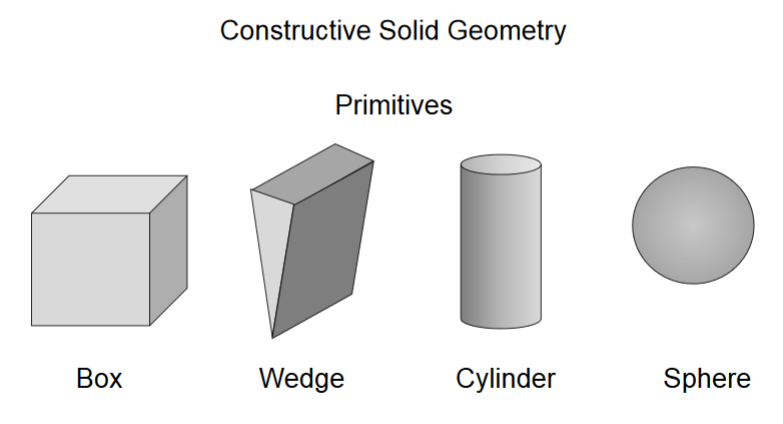
\includegraphics[width=10cm]
		{graphics/csg}}
	\caption{\label{fig:csg} Constructive Solid Geometry (CSG) Primitives}
\end{figure}
We covered a few volumetric models in the module.
\begin{enumerate}
	\item CSG: Uses primitve shapes and combines them uses set operations (union, difference, exclude, etc.) to generate new, more complex shapes.
	\item Voxels: 3D Pixels, unit cubes
	\item Octrees: Quad trees that divide in 3D space. Individual partitions are voxels
	\item Sweep: Using a 2D shape, moves that shape across a path, generating a volume in position the 2D shape occupies during its path
\end{enumerate}
One can also use implicit or parametric equations to generate shapes. Below is a list of equations that are common.
\begin{center}
	2D Circle:
	\begin{equation}
	\label{eqn:2dcirc}
	\left ( \frac{x}{r} \right )^2 + \left ( \frac{y}{r} \right )^2 = 1
	\end{equation}
	
	2D Circle - Parametric:
	\begin{equation}
	\label{eqn:2dcircpara}
	\begin{split}
	x = r\cos{\theta}  \\ y = r\sin{\theta} \\ -\pi \leq \theta \leq \pi
	\end{split}
	\end{equation}
	
	2D Ellipse - Parametric:
		\begin{equation}
	\label{eqn:2dellipsepara}
	\begin{split}
	x = r_x\cos{\theta}  \\ y = r_y\sin{\theta} \\ -\pi \leq \theta \leq \pi
	\end{split}
	\end{equation}
	
	3D Sphere:
	\begin{equation}
	\label{eqn:3dsphere}
	\left ( \frac{x}{r} \right )^2 + \left ( \frac{y}{r} \right )^2 + \left ( \frac{z}{r} \right )^2 = 1
	\end{equation}
	
	3D Ellipsoid:
	\begin{equation}
	\label{eqn:3dellipse}
	\left ( \frac{x}{r_x} \right )^2 + \left ( \frac{y}{r_y} \right )^2 + \left ( \frac{z}{r_z} \right )^2 = 1
	\end{equation}
	
	3D Sphere - Parametric:
	\begin{equation}
	\label{eqn:3dspherepara}
	\begin{split}
	x = r\cos{\phi}\cos{\theta}  \\ y = r\cos{\phi}\sin{\theta} \\ z = r\sin{\phi}\\ -\pi \leq \theta \leq \pi \\ -\pi/2 \leq \phi \leq \pi/2
	\end{split}
	\end{equation}
	
	3D Ellipsoid - Parametric:
	\begin{equation}
	\label{eqn:3dspherepara}
	\begin{split}
	x = r_x\cos{\phi}\cos{\theta}  \\ y = r_y\cos{\phi}\sin{\theta} \\ z = r_z\sin{\phi}\\ -\pi \leq \theta \leq \pi \\ -\pi/2 \leq \phi \leq \pi/2
	\end{split}
	\end{equation}
\end{center}

\subsection{Examples}
   \begin{figure}[!htb]
	\center{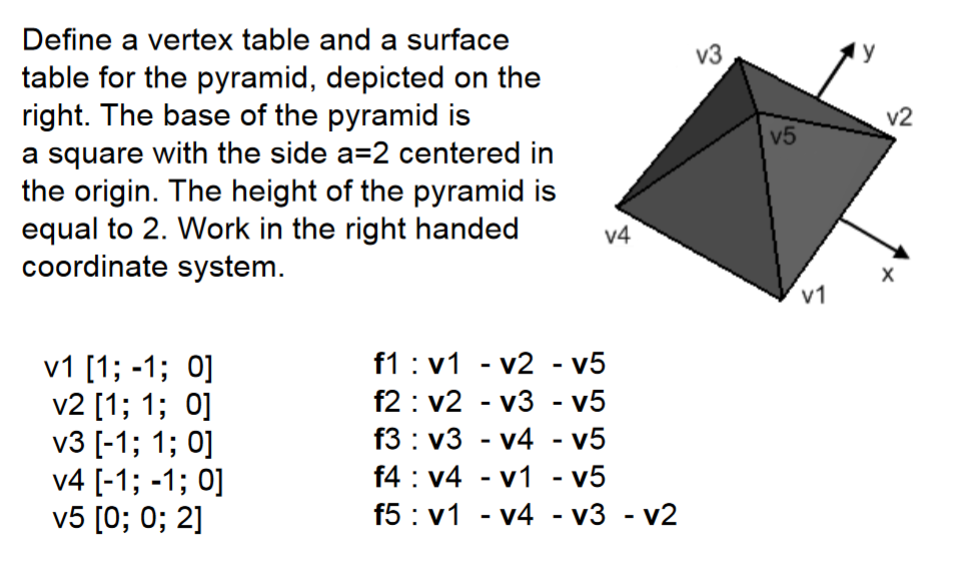
\includegraphics[width=12cm]
		{graphics/polygonTable}}
	\caption{\label{fig:pyramidPolygons} Example from Lecture}
	\end{figure}
\newpage
Further Examples are taken from quizzes and assignments
   \begin{figure}[!htb]
	\center{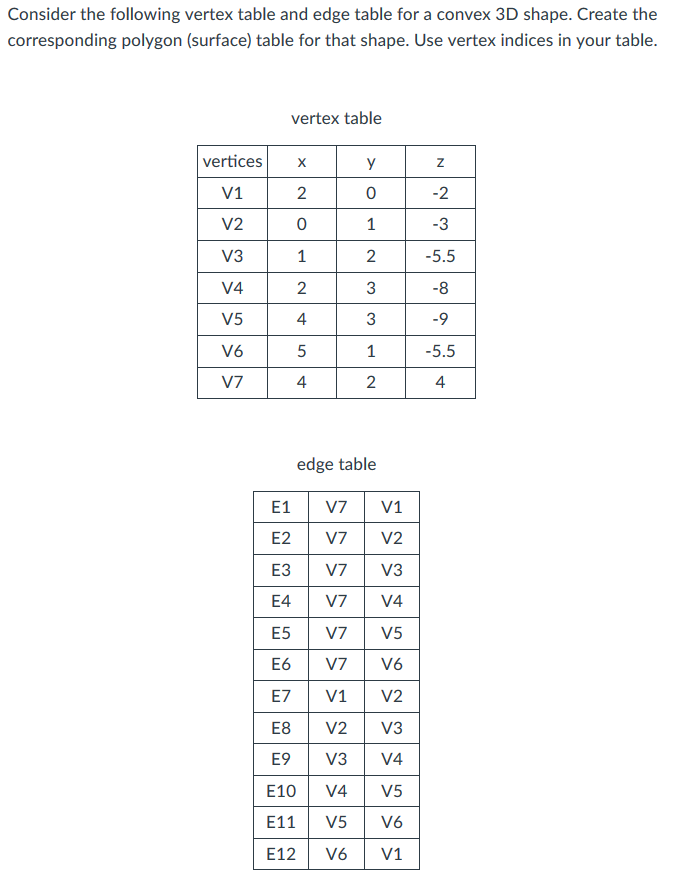
\includegraphics[width=14cm]
		{graphics/quizq1}}
	\caption{\label{fig:pyramidPolygons} Example from Quiz}
\end{figure}

Surfaces:

S1 = V1, V2, V3, V4, V5, V6

S2 = V1, V7, V2

S3 = V2, V7, V3

S4 = V2, V7, V3

S5 = V4, V7, V5

S6 = V5, V7, V6

S7 = V6, V7, V1
\subsection{Normal Vectors}
The normal vector of a surface points outwards from the surface. This is later used for lighting, projection and culling. Calculating normal vectors is a fairly simple task. For boundary polygons, the normal of a face is the cross product of two edges.
Assuming vectors A and B, the cross product is the determinant of the following matrix;

\begin{equation}
\label{eqn:crossprodMat}
\begin{bmatrix}
i & j & k\\ 
A_x & A_y & A_z\\ 
B_x & B_y & B_z
\end{bmatrix}
\end{equation}

Which can be minimized to the following (longer) equation;

\begin{equation}
\label{eqn:crossprodLine}
N = \begin{bmatrix}
A_yB_z - A_zB_y\\ 
A_zB_x - A_xB_z\\ 
A_xB_y - A_yB_x
\end{bmatrix}
\end{equation}

To know which vectors to use for A and B, simply select an edge on a surface, and you use your right hand with your thumb pointing outwards and curl your hand around in the direction until the first vector hits your hand. Alternatively, you can piece it together by looking at the figure.
  \begin{figure}[!htb]
	\center{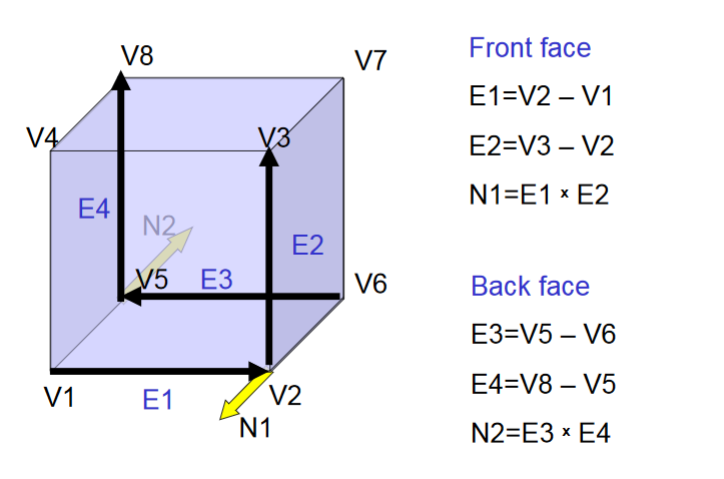
\includegraphics[width=10cm]
		{graphics/normal}}
	\caption{\label{fig:normalCube} Normal Vector of cube from lecture}
\end{figure}

\subsection{Further Sources}
	\href{https://www.tutorialspoint.com/computer_graphics/computer_graphics_surfaces.htm}{Surface Representations}
	\newline
	\href{https://www.cs.cmu.edu/afs/cs/academic/class/15462-s09/www/lec/04/lec04.pdf}{Alternate Lecture}
\newpage
\section{Transforms}
This section covers simple transformation matrices.
\subsection{Notes}
\begin{itemize}
	\item Transformation: a function that can be applied to each of the points in a geometric object to produce a new object.
	\item Translation: A geometric transform that adds a given translation amount to each coordinate of a point. Translation is used to move objects without changing their size or orientation.
	\item Rotation: A geometric transform that rotates each point by a specified angle about some point (in 2D) or axis (in 3D).
	\item Scaling: A geometric transform that multiplies each coordinate of a point by a number called the scaling factor. Scaling increases or decreases the size of an object, but also moves its points closer to or farther from the origin.
\end{itemize}
Transformations are applied to geometric objects to move them around. This is valuable when considering camera positions, or when laying out a world in a video game.
Transformations can be applied as equations for each dimensions eg. \[T_x = x + t_x\] is the new x-position when applying the translation. However, there is a lack of uniformity between different transforms, some requiring x and y more than once, others being matrices. To standardize transforms, we instead use \textit{Homogeneous Transformation Matrices}. Convert a 2D point to a 3D point by setting z = 1, and apply the transforms as matrices by replacing the variable found in each matrix template. This is an easy way of standardizing the equations, and allows for easy transforms by multiplying the transformations together before multiplying them with the point.

For example, applying a Translation {T} and then a Rotation {R} can be done by multiplying {RT} first and then multiplying the new transform matrix with the original points. This also makes it more efficient to move more than one point when they share the same transform, as it only need one multiplication per-point rather than one per-transform per-point.
\subsection{Transformation Matrices}

\begin{equation}
\label{eqn:crossprodLine}
T_{2D} = \begin{bmatrix}
1 & 0 & T_x\\ 
0 & 1 & T_y\\ 
0 & 0 & 1\\ 
\end{bmatrix}
\end{equation}

\begin{equation}
\label{eqn:crossprodLine}
S_{2D} = \begin{bmatrix}
S_x & 0 & 0\\ 
0 & S_y & 0\\ 
0 & 0 & 1\\ 
\end{bmatrix}
\end{equation}

\begin{equation}
\label{eqn:crossprodLine}
R_{2D} = \begin{bmatrix}
\cos{\theta} & -\sin{\theta} & T_x\\ 
\sin{\theta} & \cos{\theta} & T_y\\ 
0 & 0 & 1\\ 
\end{bmatrix}
\end{equation}

\begin{equation}
\label{eqn:crossprodLine}
T_{3D} =\begin{bmatrix}
1 & 0 & 0 & T_x\\ 
0 & 1 & 0 & T_y\\ 
0 & 0 & 1 & T_z\\
0 & 0 & 0 & 1 
\end{bmatrix}
\end{equation}

\begin{equation}
\label{eqn:crossprodLine}
S_{3D} = \begin{bmatrix}
S_x & 0 & 0 & 0\\ 
0 & S_y & 0 & 0\\ 
0 & 0 & S_z & 0\\
0 & 0 & 0 & 1 
\end{bmatrix}
\end{equation}

\begin{equation}
\label{eqn:crossprodLine}
R_{3D_X} = \begin{bmatrix}
1 & 0 & 0 & 0\\ 
0 & \cos{\theta} & -\sin{\theta} & 0\\ 
0 & \sin{\theta} & \cos{\theta} & 0\\
0 & 0 & 0 & 1 
\end{bmatrix}
\end{equation}

\begin{equation}
\label{eqn:crossprodLine}
R_{3D_Y} = \begin{bmatrix}
\cos{\theta} & 0 & \sin{\theta} & 0\\ 
0 & 1 & 0 & 0\\ 
-\sin{\theta} & 0 & \cos{\theta} & 0\\
0 & 0 & 0 & 1 
\end{bmatrix}
\end{equation}

\begin{equation}
\label{eqn:crossprodLine}
R_{3D_Z} = \begin{bmatrix}
\cos{\theta} & -\sin{\theta} & 0 & 0\\ 
\sin{\theta} & \cos{\theta} & 0 & 0\\ 
0 & 0 & 1 & 0\\
0 & 0 & 0 & 1
\end{bmatrix}
\end{equation}
\subsection{Examples}
\textbf{MATLAB Assignment}
\textbf{Rotating}
\begin{figure}[!hbt]
	\begin{lstlisting}
	2. Apply rotation transformation to bowl object mesh model
	%%% Define matrices for rotation of the bowl object around x, y and z axes by 20, 80 and 55 degrees respectively. 
	%%% Apply these three transformations to the original (non-transformed) bowl object in the given order 
	%%% and visualize the result using trisurf function. 
	%%% Save the result of your visualization to "2.png" file and include this file in your submission.
	rx = [1 0 0 0; 0 cosd(20) -sind(20) 0; 0 sind(20) cosd(20) 0; 0 0 0 1];
	ry = [cosd(80) 0 sind(80) 0; 0 1 0 0; -sind(80) 0 cosd(80) 0; 0 0 0 1];
	rz = [cosd(55) -sind(55) 0 0; sind(55) cosd(55) 0 0; 0 0 1 0; 0 0 0 1];
	rotated_object_vertices = rz*ry*rx*obj_v4;
	\end{lstlisting}	
\end{figure}

\textbf{Scaling}
\begin{figure}[!hbt]
	\begin{lstlisting}
%% 3. Apply scaling transformation to bowl object mesh model
%%% Define a matrix for scaling of bowl object with scaling factor f = [3.5, 1.5, 2] in direction of x, y and
%%% z axes. Apply this matrix to your original bowl object (non-transformed) and visualize the result
%%% using trisurf function. Save the result of your visualization to "3.png"? file and include this file in your
%%% submission.

scaling = [3.5 0 0 0; 0 1.5 0 0; 0 0 2 0; 0 0 0 1];
scaled_object_vertices = scaling*obj_v4;
	\end{lstlisting}	
\end{figure}
\newpage
\textbf{Translating}
\begin{figure}[!hbt]
	\begin{lstlisting}
%% 4. Apply translation transformation to bowl object mesh model
%%% Define a matrix for translation of bowl object by [-500, 50, -100] in direction of x, y and z axes. Apply
%%% this matrix to your original bowl object and visualize the result using trisurf function. Save the result
%%% of your visualization to "4.png"? file and include this file in your submission.

translate = [1 0 0 -500; 0 1 0 50; 0 0 1 -100; 0 0 0 1];
translated_object_vertices = translate*obj_v4;
	\end{lstlisting}	
\end{figure}

\textbf{3-in-1 Wombo Combo}
\begin{figure}[!hbt]
	\begin{lstlisting}
%% 5. Apply all 3 transformations defined above to your original (non-transformed) bowl object one after the other in the given order.
%%% Display transformed meshes in the figure using trisurf.
%%% Save the result of your visualisation to "5.png" file and include this file to you submission folder. 

%% Compute transformations (4x4 transformation matrices)

object_transformation = translate*scaling*rz*ry*rx;
	\end{lstlisting}	
\end{figure}
\subsection{References}
\href{http://math.hws.edu/graphicsbook/c2/s3.html}{Quick Overview}

\newpage
\section{Lighting}
This section covers things related to lighting and shading of objects in a scene.
\subsection{Notes}
\begin{itemize}
	\item Diffuse: Non-shiny illumination
	\item Specular: Shiny reflections
	\item Ambient: background illumination
\end{itemize}
\textbf{Ambient Light}
\begin{itemize}
	\item Global background light
	\item No direction
	\item Does not depend on anything
\end{itemize}
\textbf{Diffuse Light}
\begin{itemize}
	\item Parallel Light Rays originating from a source direction
	\item Contributes to Diffuse and Specular Term
\end{itemize}
\textbf{Spot Light}
\begin{itemize}
	\item Originates from a single source point
	\item Conic dispersion of light, intensity is a function of distance
	\item More realistic
\end{itemize}
\textbf{Surface Properties}
\begin{itemize}
	\item Geometry - Position, orientation
	\item Colour - reflectance and Absorption spectrum
	\item Micro-structure - defines reflectance properties
\end{itemize}
\textbf{Shading Models}
\begin{itemize}
	\item	Flat shading is the simplest shading model. Each rendered polygon has a single normal vector; shading for the entire polygon is constant across the surface of the polygon. With a small polygon count, this gives curved surfaces a faceted look.
	
	\item	Phong shading is the most sophisticated of the three. Each rendered polygon has one normal vector per vertex; shading is performed by interpolating the vectors across the surface and computing the color for each point of interest.
	
	\item	Gouraud shading is in between the two: like Phong shading, each polygon has one normal vector per vertex, but instead of interpolating the vectors, the color of each vertex is computed and then interpolated across the surface of the polygon.
\end{itemize}
  \begin{figure}[!htb]
	\center{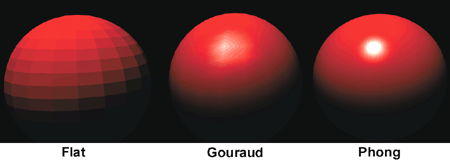
\includegraphics[width=10cm]
		{graphics/shadingModels}}
	\caption{\label{fig:normalCube} Shading Model Differences}
\end{figure}
\subsection{Phong Shading Equation}
\begin{equation}
\label{eqn:phongEqn}
\begin{split}
Colour = Ambient + Diffuse + Specular \\
Colour = I_aK_a + I_dK_d\cos{\theta_L} + I_sK_s\cos^n{\theta_S} 
\end{split}
\end{equation}

\textbf{Ambient Term}
This is very easy. It is the $K_{a}$ term multiplied with the Ambient intensity $I_{a}$.
\begin{equation}
\label{eqn:phongAmbient}
Ambient = I_aK_a
\end{equation}

\textbf{Diffuse Term}
The diffuse term is usually straight forward.. It is the $K_{d}$ term multiplied with the Light source intensity $I_{d}$. The angle $\theta$ between the light source and the normal of the surface is then computed, and the $cos(\theta)$ is multiplied to obtain the full term.
\begin{equation}
\label{eqn:phongDiffuse}
Diffuse =  I_dK_d\cos{\theta_L}
\end{equation}

\begin{figure}[!htb]
\center{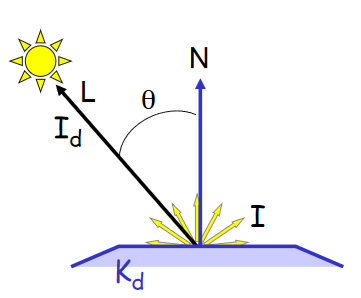
\includegraphics[width=5cm]
	{graphics/diffuse}}
\caption{\label{fig:diffuse} Diffuse term overview}
\end{figure}

\textbf{Specular Term}
The specular term needs a few more steps. It is the $K_{s}$ term multiplied with the reflected Light source intensity $I_{s}$. This is the ray that is bounced off of the surface, and is $\theta_L$ away from the normal of the surface. This intensity is multiplied by the $\cos$ of the angle $\theta_S$, the angle between the reflected ray and the line of sight from the camera. The $\cos$ is raised to the $n_{th}$ power, a factor known as a shininess factor that is usually given.

\begin{equation}
\label{eqn:phongSpecular}
Diffuse =  I_dK_d\cos^n{\theta_S}
\end{equation}
\begin{figure}[!htb]
	\center{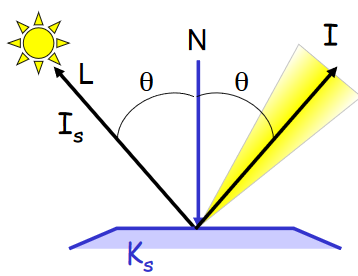
\includegraphics[width=5cm]
		{graphics/specular}}
	\caption{\label{fig:specular} Specular term overview}
\end{figure}
\newpage

\subsection{Examples}
\subsubsection{MATLAB Assignment}
\textbf{Calculating Ambient Term}
\begin{figure}[!hbt]
\begin{lstlisting}
function colour = calcAmbient_skeleton(pixel_colour_current, Ia,Ka)

% Colour at current pixel
colour = pixel_colour_current;

% TO DO: Compute colour of the pixel here and write values to the
% corresponding place in image ImA 

ambient = Ia.* Ka;
for i = 1:size(colour, 3)
colour(:,:,i) = ambient(i,i,:);
end
end
\end{lstlisting}	
\end{figure}

\textbf{Calculating Diffuse Term}
\begin{figure}[!hbt]
	\begin{lstlisting}
function colour = calcDiffuse_skeleton(pixel_colour_current, point_position, light_position, surface_normal, Id, Kd)

% Colour at current pixel
colour = pixel_colour_current;

%TO DO: Calculate light direction from light position and point position
light_direction = light_position - point_position;
%TO DO: Calculate normalised light direction
normalised_light = light_direction / norm(light_direction);
%TO DO: Calculate cos light direction, removing negative
%values
cos_light = dot(surface_normal, normalised_light);

%TO DO: Compute colour colour of the pixel here and write
% values to the corresponding place in image ImD
diffuse = Id.*(Kd.*cos_light);
for i = 1:size(colour, 3)
colour(:,:,i) = colour(:,:,i) + diffuse(i);
end
end
	\end{lstlisting}	
\end{figure}

\newpage

\textbf{Calculating Specular Term}
\begin{figure}[!hbt]
	\begin{lstlisting}
function colour = calcSpecular_skeleton(pixel_colour_current, point_position, light_position, surface_normal,normal_towardsViewer, shininess_factor, Is, Ks)

% Colour at current pixel
colour = pixel_colour_current;

%TO DO: Calculate light direction from light position and point position
light_direction = point_position - light_position;

%TO DO: Normalised light direction
normalised_light = light_direction / norm(light_direction);
%TO DO: Normal component
n = surface_normal / norm(surface_normal);
%TO DO: Reflected Ray (tangent + ray in one step) 
R = n*2*dot(n, -1*normalised_light) + normalised_light;
%TO DO: Normalised Reflected Ray
normalised_reflection = R / norm(R);
%TO DO: Calculate cos_spec, removing negative values
cos_light = dot(normal_towardsViewer, normalised_reflection);
if (cos_light < 0)
cos_light = 0;
end
%TO DO:  compute colour colour of the pixel here and write
% values to the corresponding place in image ImS
specular = Is.*(Ks.*(cos_light^shininess_factor));
for i = 1:size(colour, 3)
colour(:,:,i) = colour(:,:,i) + specular(i);
end

end
	\end{lstlisting}	
\end{figure}

\subsection{References}
\href{http://learnwebgl.brown37.net/09_lights/lights_specular.html}{WebGL Specular Term}

\newpage
\section{Projection}
This section deals with the virtual camera and how objects are projected from a proposed 'world' to a camera space.
\subsection{Notes}
\begin{itemize}
	\item View Reference Point (VRP): The centre point/position where the eyes/camera is positioned
	\item Viewing Plane: The 2D plane in which images are rendered onto in relation to the camera
	\item Gaze Vector (N): The direction vector from the VRP facing towards the viewing plane
	\item Up Vector (U): The vector perpendicular to the normal facing upwards in relation to the Gaze Vector
	\item Handedness Vector (V): The vector perpendicular to the Gaze and Up Vectors facing right in relation to the gaze vector.
	\item Camera Coordinate System: The coordinate system formed by the N, U and V vectors acting as axes
\end{itemize}
  \begin{figure}[!htb]
	\center{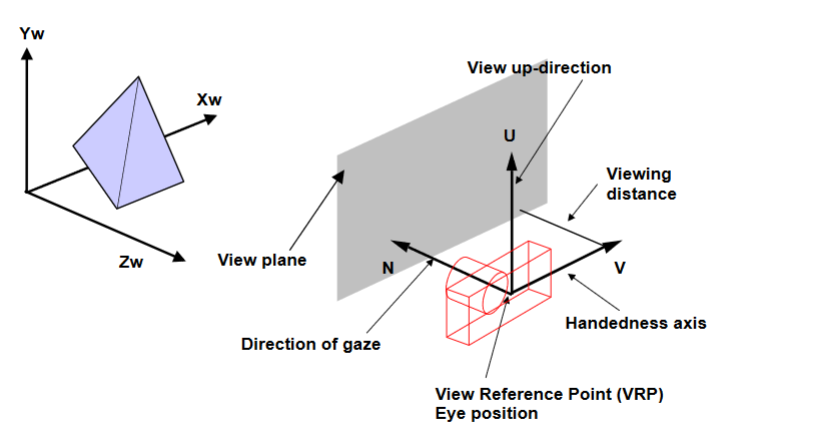
\includegraphics[width=12cm]
		{graphics/cameraDefs}}
	\caption{\label{fig:camDefs} Visualised definitions}
\end{figure}
When rendering to camera, you first need to have a World Coordinate System and objects in that world. From there, you should know VRP and the Viewing Plane. (TP is the position on the Viewing Plane the camera points to.) Using this information, we can calculate the Camera Coordinate System (N V U).
\begin{figure}[!htb]
	\centering
	U$_{temp}$ = [0 1 0]
		
	N = TP - VRP
	
	V = U$_{temp}$ x N
	
	U = N x V
\end{figure}

We use transformation matrices to move objects form the World Coordinate System to the Camera Coordinate System. Translate to the camera position, rotate to orient with the camera, then scale the x-axis $-1$ to convert to the left-hand coordinate system to avoid mirroring.

\begin{equation}
\label{eqn:tanslateCam}
T_{cam} =\begin{bmatrix}
1 & 0 & 0 & -x_{vrp}\\ 
0 & 1 & 0 & -y_{vrp}\\ 
0 & 0 & 1 & -z_{vrp}\\
0 & 0 & 0 & 1 
\end{bmatrix}
\end{equation}

\begin{equation}
\label{eqn:rotateCam}
R_{cam} =\begin{bmatrix}
\frac{V_x}{\left | \mathbf{V} \right |} & \frac{V_y}{\left | \mathbf{V} \right |} & \frac{V_z}{\left | \mathbf{V} \right |} & 0\\ 
\frac{U_x}{\left | \mathbf{U} \right |} & \frac{U_y}{\left | \mathbf{U} \right |} & \frac{U_z}{\left | \mathbf{U} \right |} & 0\\ 
\frac{N_x}{\left | \mathbf{N} \right |} & \frac{N_y}{\left | \mathbf{N} \right |} & \frac{N_z}{\left | \mathbf{N} \right |} & 0\\ 
0 & 0 & 0 & 1 
\end{bmatrix}
\end{equation}

\begin{equation}
\label{eqn:scaleCam}
S_{cam} = \begin{bmatrix}
-1 & 0 & 0 & 0\\ 
0 & 1 & 0 & 0\\ 
0 & 0 & 1 & 0\\
0 & 0 & 0 & 1 
\end{bmatrix}
\end{equation}


\begin{itemize}
	\item Centre of Project (COP): The view point the perspective is drawn from, usually the camera position
	\item Perspective Projection: Objects further away from the COP are scaled smaller
	\item Orthographic Projection: All objects are on the same scale, regardless of COP
\end{itemize}
\begin{figure}[!htb]
\center{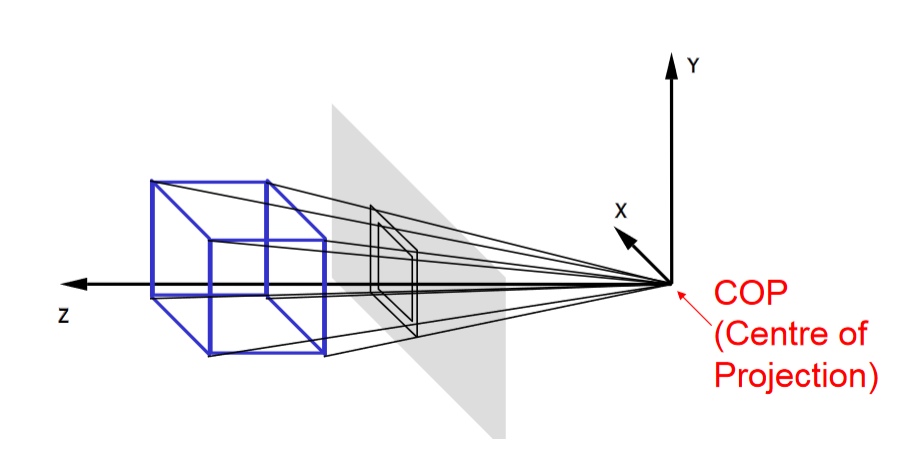
\includegraphics[width=12cm]
	{graphics/cop}}
\caption{\label{fig:cop} Projection Lines meet at the COP}
\end{figure}
The centre of project can be placed at either the centre/origin of the viewing coordinate system with the viewing plane on the positive z size, or the negative z side with the viewing plane placed on the centre/origin of the viewing coordinate system. Depending on which method is chosen, the computation differs slightly.

\subsubsection{COP at Z=0}
\begin{figure}[!htb]
	\center{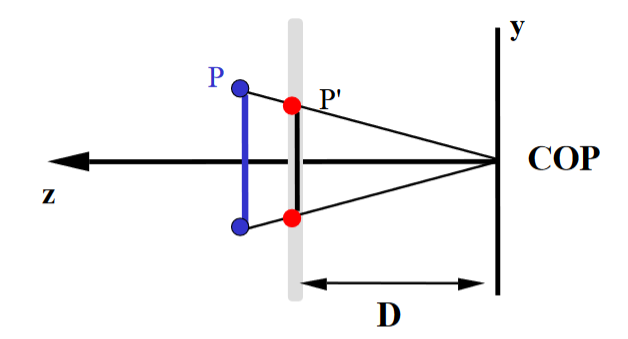
\includegraphics[width=9cm]
		{graphics/trianglesZ0}}
	\caption{\label{fig:trianglesZ0} COP = 0}
\end{figure}
\begin{equation}
\label{eqn:proj0}
P_{per} = \begin{bmatrix}
1 & 0 & 0 & 0\\ 
0 & 1 & 0 & 0\\ 
0 & 0 & 1 & 0\\
0 & 0 & 1/\mathbf{D} & 0 
\end{bmatrix}
\end{equation}
Where \textbf{D} is the distance from the COP and the viewing plane. The generated matrix after multiplication is not homogenous; to convert it to homogenous form we simply divide all terms by the 4th term, which equates to \[z/D\]

With the perspective project matrix, we can create a general form for moving the object from the World Space to the Camera Space.
\begin{equation}
\label{eqn:worldToCam1}
C = P_{per} * S_{cam} * R_{cam} * T_{cam}
\end{equation}
With the new vector converted to homogenous coordinates after applying $C$.
All new coordinates should also have their Z coordinate equal to te Z coordinate of the viewing plane.

\textbf{COP at Z<0}
When the viewing plane is at the origin, $P_{per}$ changes slightly.
\begin{equation}
\label{eqn:proj1}
P_{per} = \begin{bmatrix}
1 & 0 & 0 & 0\\ 
0 & 1 & 0 & 0\\ 
0 & 0 & 1 & 0\\
0 & 0 & 1/\mathbf{D} & 1 
\end{bmatrix}
\end{equation}
Converting to homogenous would also be slightly different, but will still be fairly simple.
All Z coordinates should end up at Z=0.

\subsection{Examples}

The questions here are from the quiz.

Consider the following vertex coordinates:
\begin{figure}[!hbt]
	\centering
	V1 = [0, 10, 0]
	
	V2 = [5, 0, 5]
	
	V3 = [15, 5, 0]
	
	V4 = [5, 10, 15]
\end{figure}

Define the viewing (camera) coordinate system by computing its axes, i.e., direction of gaze N, handedness vector V, and vector U which is the correct up-vector. Camera view reference point is VRP = [60, 30, 100], and the target point TP is at the origin ([0, 0, 0]). The camera coordinate system should be defined in the same way as it is shown in the lecture slides: using temporary up vector of [0,1,0] to compute handedness and up vectors of the camera.
\begin{enumerate}
	\item What is the direction of the gaze vector?
	\item What is the handedness vector?
	\item What is the up vector?
	\item Compute the matrix $C_1$ to transform an object from the world coordinate system to the camera coordinate system (without project).
	\item Compute the matrix $C_2$ to transform an object from the world coordinate system to the camera coordinate system with the COP at the origin and the viewing plane at z= +40.
	\item Compute the positions of the final transformed vertices.
\end{enumerate}
\newpage
\textbf{Answers to the previous questions}
\newline
\begin{enumerate}
	\item $N = [-0.50, -0.25, -0.83]$
	\item $V = [-0.86, 0, 0.51]$
	\item $U = [-0.13, 0.97, -0.21]$
	\item $C_1$ = $\begin{bmatrix}
		0.857 & 0 & -0.514 & 0\\ 
		-0.128 & 0.968 & -0.214 & 0\\ 
		-0.498 & -0.249 & -0.830 & 120\\
		0 & 0 & 0 & 1 
	\end{bmatrix}$
		\item $C_2$ = $\begin{bmatrix}
	0.857 & 0 & -0.514 & 0\\ 
	-0.128 & 0.968 & -0.214 & 0\\ 
	-0.498 & -0.249 & -0.830 & 120\\
	-0.013 & -0.006 & -0.021 & 3.010 
	\end{bmatrix}$
	\item $V_1 = [0.00, 3.29, 40.0]$
	
	$V_2 = [0.60, -0.60, 40]$
	
	$V_3 = [4.61, 1.05, 40]$
	
	$V_4 = [-1.33, 2.27, 40]$
\end{enumerate}
\subsection{References}
No external references were needed on this section.
\newpage
\section{Misc. Definitions}
This section covers general algorithms and definitions from Rendering to Texture Mapping. Since the exam will focus more on the previous parts for the more technical questions, this part will mostly be structured as a set of definitions.

\subsection{Rasterisation}
\begin{itemize}
	\item Rasterisation: Converting an object from vector world coordinates to a raster image to display
	\item Digital Differential Analyzer (DDA): Rasterisation algorithm, interpolates values in an interval by computing separate equations for $(x,y)$. Is expensive and inefficient.
	\item Bresenham Algorithm: Incremental, integer only algorithm. Has many implementations.
	\item Antialiasing: utilizes blending techniques to blur the edges of the lines and provide the viewer with the illusion of a smoother line. 
\end{itemize}
Circles can be plotted either directly with a circle equation, directly with polar coordinates, or using Bresenhams by looping across a set of values until all values on a circle are plotted. Bresenham and Polar methods abuse the symmetry of a circle's points.
\begin{figure}[!htb]
	\center{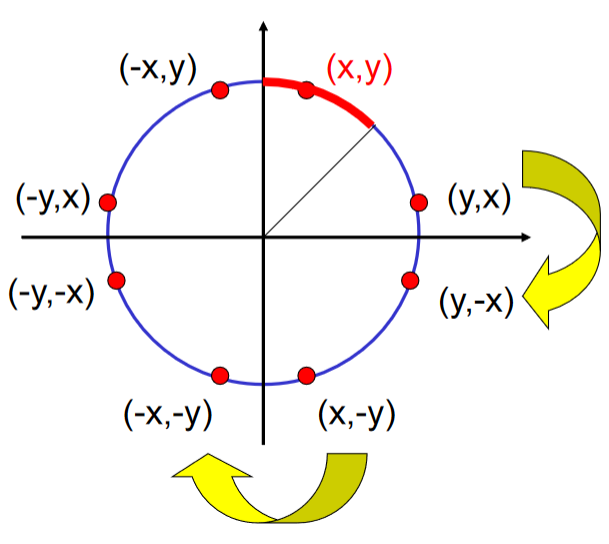
\includegraphics[width=6cm]
		{graphics/circle}}
	\caption{\label{fig:circleRaster} Symmetry of circle}
\end{figure}
\subsection{Texture Mapping}
Texture mapping can be defined as using an image and pasting the image onto a geometric model. There are three types of Texture Mapping.
\begin{enumerate}
	\item Texture Image: uses iamges to fill inside polygons; inverse mapping using an intermediate surface
	\item Environment/Reflection: uses a picture of the scene for texture maps
	\item Bump: Emulates altering normal vectors during render process
\end{enumerate}
\begin{figure}[!htb]
	\center{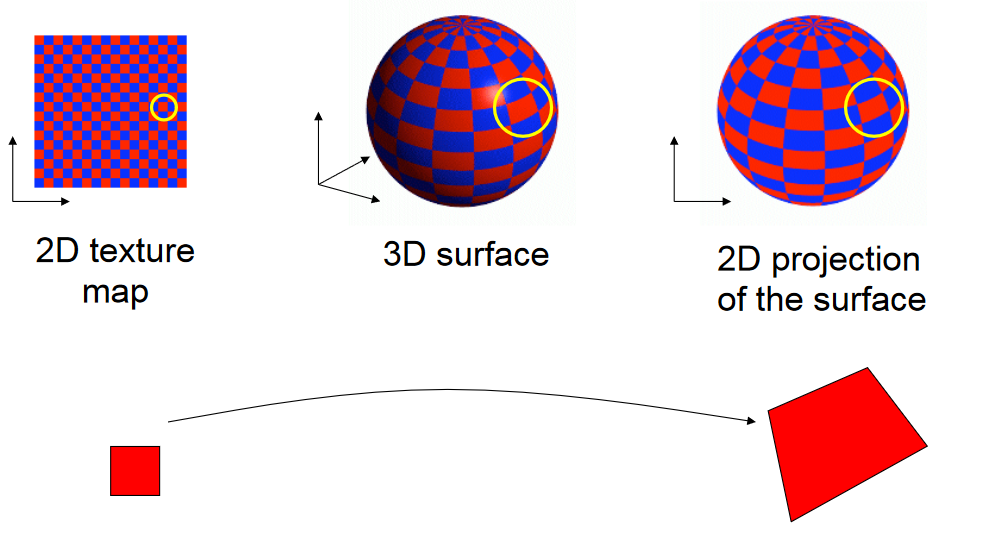
\includegraphics[width=5cm]
		{graphics/imageMapping}}
	\caption{\label{fig:imageMap} Image Mapping flow}
\end{figure}

When it comes to image mapping, there are two main methods.
\begin{enumerate}
	\item Forward: copy pixel at source $(u,v)$ to image destination $(r, c)$. Its easy to compute but leaves holes.
	\item Backward: for image pixels $(r,c)$, grab texture pixel $(u,v)$. Harder to compute but looks better.
\end{enumerate}
Environment mapping uses the direction of te reflected ray to index a texture map rather than using the ray projected to its surface. This approach isn't completely accurate as it assumes all reflected rays begin from the same point and that all objects in a scene are the same distance from that point.

Bump mapping is a method used to make a surface look rough. There are two variants.
\begin{enumerate}
	\item Displacement Mapping: Height filed is used to perturb surface point along the direction of its surface normal. Inconvenient to implement since map must perturb geometry of model.
	\item Bump Mapping: A perturbation is applied to the surface normal according to the corresponding value in the map. Convenient to implement as it automatically changes the shading parameters of a surface.
\end{enumerate}

There is also mip-mapping. Mapping can cause aliasing to occur; mip-mapping is an anti-aliasing technique that stores texture as a pyramid of progressive resolution images, filtered down from the original. The further away a point is to be rendered, the lower lower resolution MIP-map is used.
\begin{figure}[!htb]
	\center{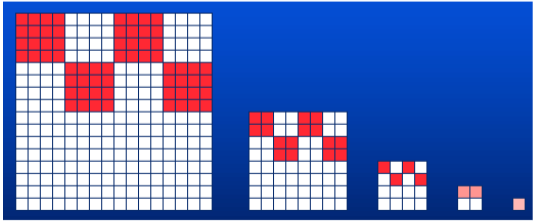
\includegraphics[width=7cm]
		{graphics/mipmap}}
	\caption{\label{fig:imageMap} MIP-map examples}
\end{figure}
\subsection{Hidden Surface Removal}
\begin{enumerate}
	\item Object-space method (OS): Operate on 3D Object entities.(vertices, edges, surfaces)
	\item Image-sped (IS): Operate on 2D images (pixels)
\end{enumerate}
There are a few algorithms to go over.
\begin{itemize}
	\item Polygon Culling: removes all surfaces pointing away from the viewer; renders only what is visible; can be done by comparing if the z-value of the surface normal has the same sign as the z-value of the gaze vector. (If same, remove surface)
	\item Z-buffer Algorithm: Test visibility of surfaces one point at a time. Easy to implement, fits well with render pipeling, but some inefficiency with large distances. Standard algorithm in many packages, eg. OpenGL
	\item Painter's Algorithm: OS algorithm; Draw surfaces from back to front. Problems occur with overlapping polygons; as it will always render an object either above or below absolutely.
	\item Depth Sort: Painter's extension; sorts objects by depth like painters, but resolves overlap issues, splitting polygons if necessary. Does overlap/collision testing and splits on intersection point.
\end{itemize}
\newpage
\subsection{Splines}
Splines are smooth curves generated from an input set of user-specified control points.
\begin{figure}[!htb]
	\center{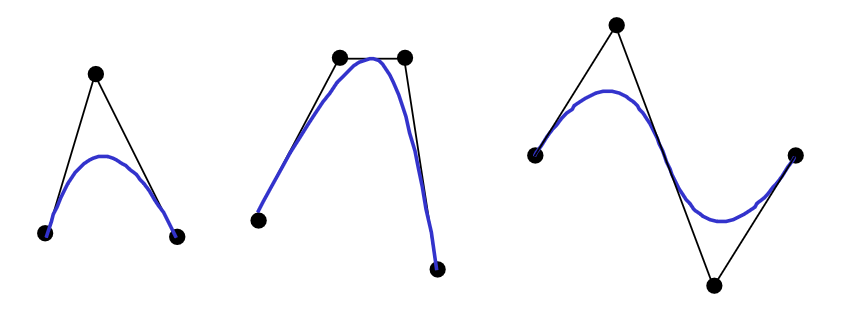
\includegraphics[width=7cm]
		{graphics/splines}}
	\caption{\label{fig:spline}Splines with different control points}
\end{figure}

Bezier curves are generated by forming a set of polynomial functions formed from the coordinates of the control points. In parametric form, a Bezier Function $P(u)$ can be represented as \[P(u) = \sum_{k=0}^{n}p_kB_{kn}(u)\]
There are many ways to formulate Bezier curves. One such method is the de Casteljau algorithm. This algorithm describes the curve as a recursive series of linear interpolations. We draw lines between each of our control points in order, then continuously Lerp (linearly interpolate) each of the points generated by the previous Lerp until a curve is formed.
\newline
\newline
Bezier curve shape is influenced by all of its control points. There are B-splines that are only influenced by up to four of the nearest control points. This allows for interesting shapes without the inefficient calculations from insanely high polynomial Bezier curves.
\newline
\newline
Bezier surfaces are similar to Bezier curves, but instead of just one parameter $t$, there are two parameters $s$ and $t$, and instead of a curve, it is a surface mesh.


\newpage